\documentclass[a4paper]{article}
\usepackage[utf8]{inputenc}
\usepackage{amsmath}
\usepackage{amsfonts}
\usepackage{amssymb}
\usepackage{graphicx}
\usepackage{geometry}
\usepackage[english]{babel}
\usepackage{enumitem}%can be used for automatic numbering of requirements/tests.
\usepackage{hyperref}
\usepackage[colorinlistoftodos]{todonotes}
\usepackage{color} % Used to write in red,blue,green etc.
\usepackage{float}
\usepackage[titletoc]{appendix}
\usepackage{pdfpages} % Append pdf files

\title{SVVR - Software Verification and Validation Report}
\newcommand{\version}{v0.9}
\newcommand{\SVVR}{PUSS154217}
\author{Testgroup, Team 2}

\newcommand{\testdate}{NOT SET}

%-------------------------TITLE-----------------------------------------

\begin{document}
\begin{titlepage}
\newgeometry{left=2cm,top=1cm,right=2cm}
\newcommand{\HRule}{\rule{\linewidth}{0.5mm}}

\begin{minipage}{0.5\textwidth}
\begin{flushleft} % Responsible persons, write on separate lines
\textit{Responsible for this document:}\\
Oskar Fällström %Not entirely sure who this should be, possibly project leaders as well?
\end{flushleft}
\end{minipage}
~
\begin{minipage}{0.4\textwidth}
\begin{flushright}
\SVVR\ \version\ %Dokumentnummer enl. projekthandledning s. 22-23 och insidan av pärmen
\today
\end{flushright}
\end{minipage}\\[3cm]

\centering
\textsc{\LARGE Team 2}\\[0.5cm]

\HRule \\[0.4cm]
{ \huge \bfseries Software Verification and Validation Report}\\[0.4cm] % Title of your document
\HRule \\[1.5cm]

\vfill
\begin{flushleft}
\textit{Authors of this document:}\\
Måns Andersson \\
Hanna Autio \\
Moa Eklöf \\
Oskar Fällström \\
Ulf Hörndahl \\
Jonathan Lundholm
\end{flushleft}	


\end{titlepage}
\pagenumbering{gobble}

\begin{center}
\textit{\large Version History}

    \begin{tabular}{ | l | l | l | p{5cm} |}
    \hline
    \textbf{Version}		& \textbf{Date}		& \textbf{Responsible}					& \textbf{Description}					\\ \hline
    0.0						& 2015-10-01 			& UH									& Document created						\\ \hline
    0.9						& 2015-10-13			& HA									& Modified according to informal review\\ \hline
    \end{tabular}
\end{center}

\setcounter{tocdepth}{2}
\tableofcontents
\newpage
\pagenumbering{arabic}


%--------------------Reference Documents ---------------------------------------
\section*{Reference Documents}
\begin{enumerate}
\item PUSS154212 - System Requirements Specification v1.2 \label{refdocs:srs} 
\item Programvaruutveckling för Stora System - Projekthandledning v2.2 \newline (\textit{Institutionen för datavetenskap}, Lunds Univeritet 2015) \label{refdocs:projekthandledning}
\item PUSS154213 - Software Verification and Validation Specification v1.4 \label{refdocs:SVVS}
\item PUSS154253 - Test Matrices for SVVS v1.1 \label{refdocs:matrices}
\item PUSS154215 - Software Verification and Validation Instruction v1.4 \label{refdocs:SVVI}
\end{enumerate}

%--------------------Introduction ---------------------------------------
\section{Known Bugs}

\subsection{Backend}

\subsection{Other}

\clearpage
\section{Functional Tests}
Below are the test protocols from the function tests.

\subsection{MyDevices View}

\renewcommand{\testdate}{151005}
\textbf{ Tests performed \testdate}
\begin{center}
  		\begin{tabular}{| p{3cm} | p{5cm} | p{5cm} |}
    		\hline
	    	\textbf{Testcase}			& \textbf{Pass/No Pass} 	& \textbf{Comment} \\ \hline
    		A.1.1		 						& Pass 								&  \\\hline
    		A.1.2		 						& Pass 								& 				 \\	\hline
    		A.1.3		 						& No Pass 							& The list is not scrollable with the available devices		 \\	\hline
    		A.1.4		 						& Pass 								& 				 \\	\hline
    		A.1.5		 						& Pass 								& 				 \\	\hline
    		A.1.6		 						& Pass 								& 				 \\	\hline
    		A.1.7		 						& No Pass 							& Wrong name of sensor 				 \\	\hline
    		A.1.8		 						& Pass 								& 				 \\	\hline
    		A.1.9		 						& Pass 								& 				 \\	\hline
    		A.1.10	 							& Pass 								& 				 \\	\hline
    		A.1.11	 							& Pass 								& 				 \\	\hline
    		A.1.12	 							&  									& Postponed				 \\	\hline 		
 		 \end{tabular}
\end{center}
	
\renewcommand{\testdate}{151008}
\textbf{ Tests performed \testdate}
\begin{center}
  		\begin{tabular}{| p{3cm} | p{5cm} | p{5cm} |}
    		\hline
	    	\textbf{Testcase}			& \textbf{Pass/No Pass} 	& \textbf{Comment} \\ \hline
    		A.1.1		 						& Pass  										&   \\ \hline
    		A.1.2		 						& Pass 										& 				 \\	\hline
    		A.1.3		 						& Pass 										& 				 \\	\hline
    		A.1.4		 						& Pass 										& 				 \\	\hline
    		A.1.5		 						& Pass 										& 				 \\	\hline
    		A.1.6		 						& Pass 										& 				 \\	\hline
    		A.1.7		 						& Pass 										& 				 \\	\hline
    		A.1.8		 						& Pass 										& 				 \\	\hline
    		A.1.9		 						& Pass 										& 				 \\	\hline
    		A.1.10	 							& Pass 										& 				 \\	\hline
    		A.1.11	 							& Pass 										& 				 \\	\hline
 		 \end{tabular}
\end{center}
	

\subsection{Sensor View}

\renewcommand{\testdate}{151005}
\textbf{Tests performed \testdate}
	\begin{center}
  		\begin{tabular}{| p{3cm} | p{5cm} | p{5cm} |}
    		\hline
	    	\textbf{Testcase}			& \textbf{Pass/No Pass} 	& \textbf{Comment} \\ \hline
    		A.2.1		 						& Pass 								&  				\\ \hline
    		A.2.2		 						& Pass  							& 				 \\	\hline
    		A.2.3		 						& No Pass 							& The status light of the sensor is off (postcondition 2)				 \\	\hline
    		A.2.4		 						& Pass  							& 				 \\	\hline
    		A.2.5		 						& Pass 								& 			 \\	\hline
    		A.2.6		 						& Pass 								& 				 \\	\hline
    		A.2.7		 						& Pass 								& 				 \\	\hline
    		A.2.8		 						& No Pass 							& Even without internet connection the app displays a value (postcondition 1)			 \\	\hline
    		A.2.9		 						& No Pass 							& (postcondition 1)				 \\	\hline
    		A.2.10	 							& Pass 								& 				 \\	\hline
    		A.2.11	 							& Pass 								& 				 \\	\hline
    		A.2.12	 							& Pass 								& 				 \\	\hline
 		 \end{tabular}
	\end{center}
\renewcommand{\testdate}{151008}
\textbf{Tests performed \testdate}
	\begin{center}
  		\begin{tabular}{| p{3cm} | p{5cm} | p{5cm} |}
    		\hline
	    	\textbf{Testcase}			& \textbf{Pass/No Pass} 	& \textbf{Comment} \\ \hline
    		A.2.1		 						& Pass 										&  				\\ \hline
    		A.2.2		 						& Pass 										& 				 \\	\hline
    		A.2.3		 						& No Pass 										& Status lamp does not correspond to the device status.				 \\	\hline
    		A.2.4		 						& Pass 										& 				 \\	\hline
    		A.2.5		 						& Pass 										& 				 \\	\hline
    		A.2.6		 						& Pass 										& 				 \\	\hline
    		A.2.7		 						& Pass 										& 				 \\	\hline
    		A.2.8		 						& No Pass 										& Wrong error message.				 \\	\hline
    		A.2.9		 						& No Pass 										& Status lamp does not correspond to the device status.				 \\	\hline
    		A.2.10	 							& Pass 										& 				 \\	\hline
    		A.2.11	 							& Pass 										& 				 \\	\hline
    		A.2.12	 							& Pass 										& 				 \\	\hline
    		A.2.13	 							& No Pass 											&  Wrong error message.				 \\	\hline
 		 \end{tabular}
	\end{center}

\subsection{Light Bulb View}
\renewcommand{\testdate}{151005}
\textbf{ Tests performed \testdate} \\
The protocol below correspond to the tests in PUSS154213 v1.2. They were performed as specified in PUSS154215 v1.0.
\begin{center}
  	\begin{tabular}{| p{3cm} | p{5cm} | p{5cm} |}
    		\hline
	    	\textbf{Testcase}			& \textbf{Pass/No Pass} 	& \textbf{Comment} \\ \hline
    		A.3.1		 					& Pass  							&  				\\ \hline
    		A.3.2		 					& Pass 							& 				 \\	\hline
    		A.3.3		 					& Pass 							& 				 \\	\hline
    		A.3.4		 					& No Pass 					& It is not possible to input capital letters (postcondition 2)				 \\	\hline
    		A.3.5		 					& Pass 							& 				 \\	\hline
    		A.3.6		 					& Pass 							& 				 \\	\hline
    		A.3.7		 					& No Pass 							& Failed on configuration 1,2,3,4,5				 \\	\hline
    		A.3.8		 					& No Pass 							& Capital letters not recognized, fail on all configurations				 \\	\hline
    		A.3.9		 					& Pass 							& 				 \\	\hline
    		A.3.10	 						& Pass 							& 				 \\	\hline
    		A.3.11	 						& No Pass 							& No error message				 \\	\hline
    		A.3.12	 						& Pass 							& 				 \\	\hline
    		A.3.13	 						& Pass						& 				 \\	\hline
    		A.3.14	 						& No Pass 							& In landscape mode: fail on instructions 3,4 and 5 (items not visible).   				 \\	\hline
 	\end{tabular}
\end{center}
\renewcommand{\testdate}{150108}
\textbf{ Tests performed \testdate} \\
The protocol below correspond to the tests in PUSS154213 v1.4. They were performed as specified in PUSS154215 v1.3.
\begin{center}
  	\begin{tabular}{| p{3cm} | p{5cm} | p{5cm} |}
    		\hline
	    	\textbf{Testcase}			& \textbf{Pass/No Pass} 	& \textbf{Comment} \\ \hline
    		A.3.1		 						& Pass 										&  				\\ \hline
    		A.3.2		 						& Pass 										& 				 \\	\hline
    		A.3.3		 						& Pass 										& 				 \\	\hline
    		A.3.4		 						& Pass 										& 				 \\	\hline
    		A.3.5		 						& Pass 										& 				 \\	\hline
    		A.3.6		 						& Pass 										& 				 \\	\hline
    		A.3.7		 						& No Pass 										& Failed on configuration 6				 \\	\hline
    		A.3.8		 						& Pass 										& 				 \\	\hline
    		A.3.9		 						& Pass 										& 				 \\	\hline
    		A.3.10	 							& Pass 										& 				 \\	\hline
    		A.3.11	 							& Pass 										& 				 \\	\hline
    		A.3.12	 							& Pass 										& 				 \\	\hline
    		A.3.13	 							& Pass 										& 				 \\	\hline
    		A.3.14	 							& Pass 										& 				 \\	\hline
 	\end{tabular}
\end{center}

\newpage
\section{System Tests}
Below are the test protocols from the system tests.

\subsection{Tests for Use Cases}
\renewcommand{\testdate}{2015-10-05}
\textbf{ Tests performed \testdate} \\
The protocol below correspond to the tests in PUSS154213 v1.2. They were performed as specified in PUSS154215 v1.0.
\begin{center}
  		\begin{tabular}{| p{3cm} | p{5cm} | p{5cm} |}
    		\hline
	    	\textbf{Testcase}			& \textbf{Pass/No Pass} 	& \textbf{Comment} \\ \hline
    		B.1.1		 						& Pass 										&  				\\ \hline
    		B.1.2		 						& No Pass 										& Failed on postconditions 1,2. 				 \\	\hline
    		B.1.3		 						& Pass 										& 				 \\	\hline
    		B.1.4		 						& Pass 										& 				 \\	\hline
    		B.1.5		 						& Pass 										& 				 \\	\hline
    		B.1.6		 						& Pass 										& 				 \\	\hline
    		B.1.7		 						& Pass 										& 				 \\	\hline
    		B.1.8		 						& Pass 										& 				 \\	\hline
    		B.1.9		 						& No Pass 										& Impossible to determine the status of the sensor device. 				 \\	\hline
    		B.1.10	 							& No Pass 										& Impossible to determine the status of the sensor device.				 \\	\hline
    		B.1.11	 							& Pass 										& 				 \\	\hline
    		B.1.12	 							& Pass 										& 				 \\	\hline
    		B.1.13	 							& No Pass 										& Wrong error message.				 \\	\hline
    		B.1.14	 							& Pass 										& 				 \\	\hline
    		B.1.15	 							& Pass 										& 				 \\	\hline
    		B.1.16	 							& Pass 										& 				 \\	\hline
    		B.1.17	 							& Pass 										& 				 \\	\hline
    		B.1.18	 							& Pass 										& 				 \\	\hline
    		B.1.19	 							& No Pass 										& Failed on postcondition 1. 				 \\	\hline
    		B.1.20	 							& No Pass 										& Failed on postcondition 1.				 \\	\hline
    		B.1.21	 							& Pass 										& 				 \\	\hline
    		B.1.22	 							& Pass 										& 				 \\	\hline
    		B.1.23	 							& Pass 										& 				 \\	\hline
    		B.1.24	 							& Pass 										& 				 \\	\hline
    		B.1.25	 							& No Pass 										& Wrong error message.				 \\	\hline
 		 \end{tabular}
	\end{center}
\renewcommand{\testdate}{151008}
\textbf{ Tests performed \testdate}
\begin{center}
  		\begin{tabular}{| p{3cm} | p{5cm} | p{5cm} |}
    		\hline
	    	\textbf{Testcase}			& \textbf{Pass/No Pass} 	& \textbf{Comment} \\ \hline
    		B.1.1		 						& Pass 										&  				\\ \hline
    		B.1.2		 						& Pass 										& 				 \\	\hline
    		B.1.3		 						& Pass 										& 				 \\	\hline
    		B.1.4		 						& Pass 										& 				 \\	\hline
    		B.1.5		 						& Pass 										& 				 \\	\hline
    		B.1.6		 						& Pass 										& 				 \\	\hline
    		B.1.7		 						& Pass 										& 				 \\	\hline
    		B.1.8		 						& Pass 										& 				 \\	\hline
    		B.1.9		 						& Pass 										& 				 \\	\hline
    		B.1.10	 							& Pass 										& 				 \\	\hline
    		B.1.11	 							& Pass 										& 				 \\	\hline
    		B.1.12	 							& No Pass 										& Does not display the correct values after pressing get.				 \\	\hline
    		B.1.13	 							& Pass 										& 				 \\	\hline
    		B.1.14	 							& Pass 										& 				 \\	\hline
    		B.1.15	 							& No Pass 										& Wrong error message.				 \\	\hline
    		B.1.16	 							& Pass 										& 				 \\	\hline
    		B.1.17	 							& No Pass								& Wrong error message				 \\	\hline
    		B.1.18	 							& Pass 										& 				 \\	\hline
    		B.1.19	 							& No Pass 										& No error message				 \\	\hline
    		B.1.20	 							& No Pass 										& No error message \\ \hline
    		B.1.21	 							& Pass 										& \\ \hline
    		B.1.22	 							& Pass										&  \\ \hline
    		B.1.23	 							& Pass											&  \\ \hline
    		B.1.24	 							& Pass											&  \\ \hline
    		B.1.25	 							& Pass											&  \\ \hline
 		 \end{tabular}
	\end{center}

\subsection{Quality Tests}
\renewcommand{\testdate}{2015-10-05}
\textbf{Tests performed \testdate} \\
The protocol below correspond to the tests in PUSS154213 v1.2. They were performed as specified in PUSS154215 v1.0.
\begin{center}
  		\begin{tabular}{| p{3cm} | p{5cm} | p{5cm} |}
    		\hline
	    	\textbf{Testcase}			& \textbf{Pass/No Pass} 	& \textbf{Comment} \\ \hline
    		B.2.1		 						& 									& Postponed 				\\ \hline
    		B.2.2		 						& No Pass 										& Failed at step 7.				 \\	\hline
    		B.2.3		 						& No Pass 										& No error messages generated.				 \\	\hline
 		\end{tabular}
\end{center}
\renewcommand{\testdate}{2015-10-08}
\textbf{Tests performed \testdate} \\
The protocol below correspond to the tests in PUSS154213 v1.4. They were performed as specified in PUSS154215 v1.3.
\begin{center}
  		\begin{tabular}{| p{3cm} | p{5cm} | p{5cm} |}
    		\hline
	    	\textbf{Testcase}			& \textbf{Pass/No Pass} 	& \textbf{Comment} \\ \hline
    		B.2.1		 						&  												& Postponed 				\\ \hline
    		B.2.2		 						& No Pass 										& Failed in instructions: 2 and 7				 \\	\hline
    		B.2.3		 						& No Pass 										& Failed to generate error messages in instructions: 2,4,5,6,7 				 \\	\hline
 		\end{tabular}
\end{center}

\newpage
\section{Review Protocols - Informal}
Here is a collection of the protocols from the informal reviews.

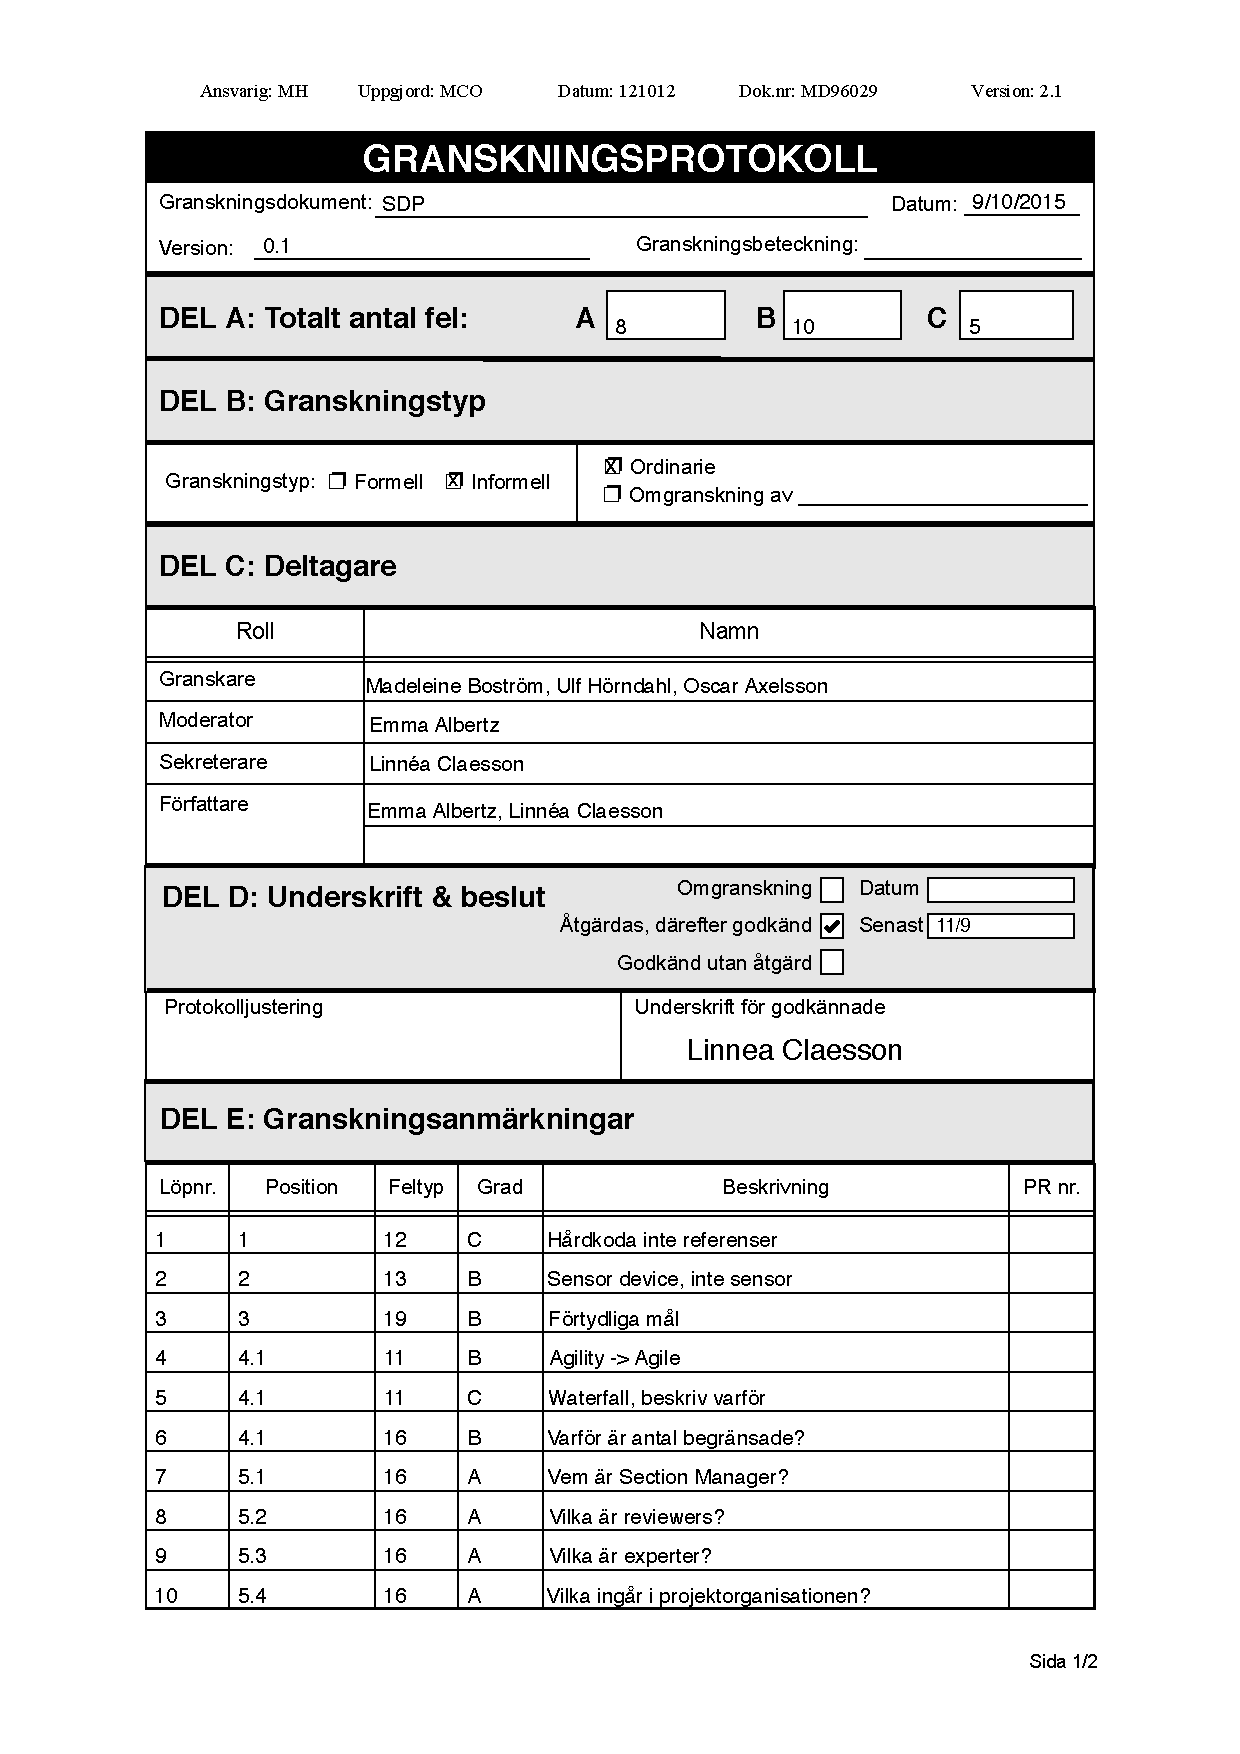
\includepdf[pages=-]{Reviews/Informal/Informal_Review_Protocol_SDP.pdf}

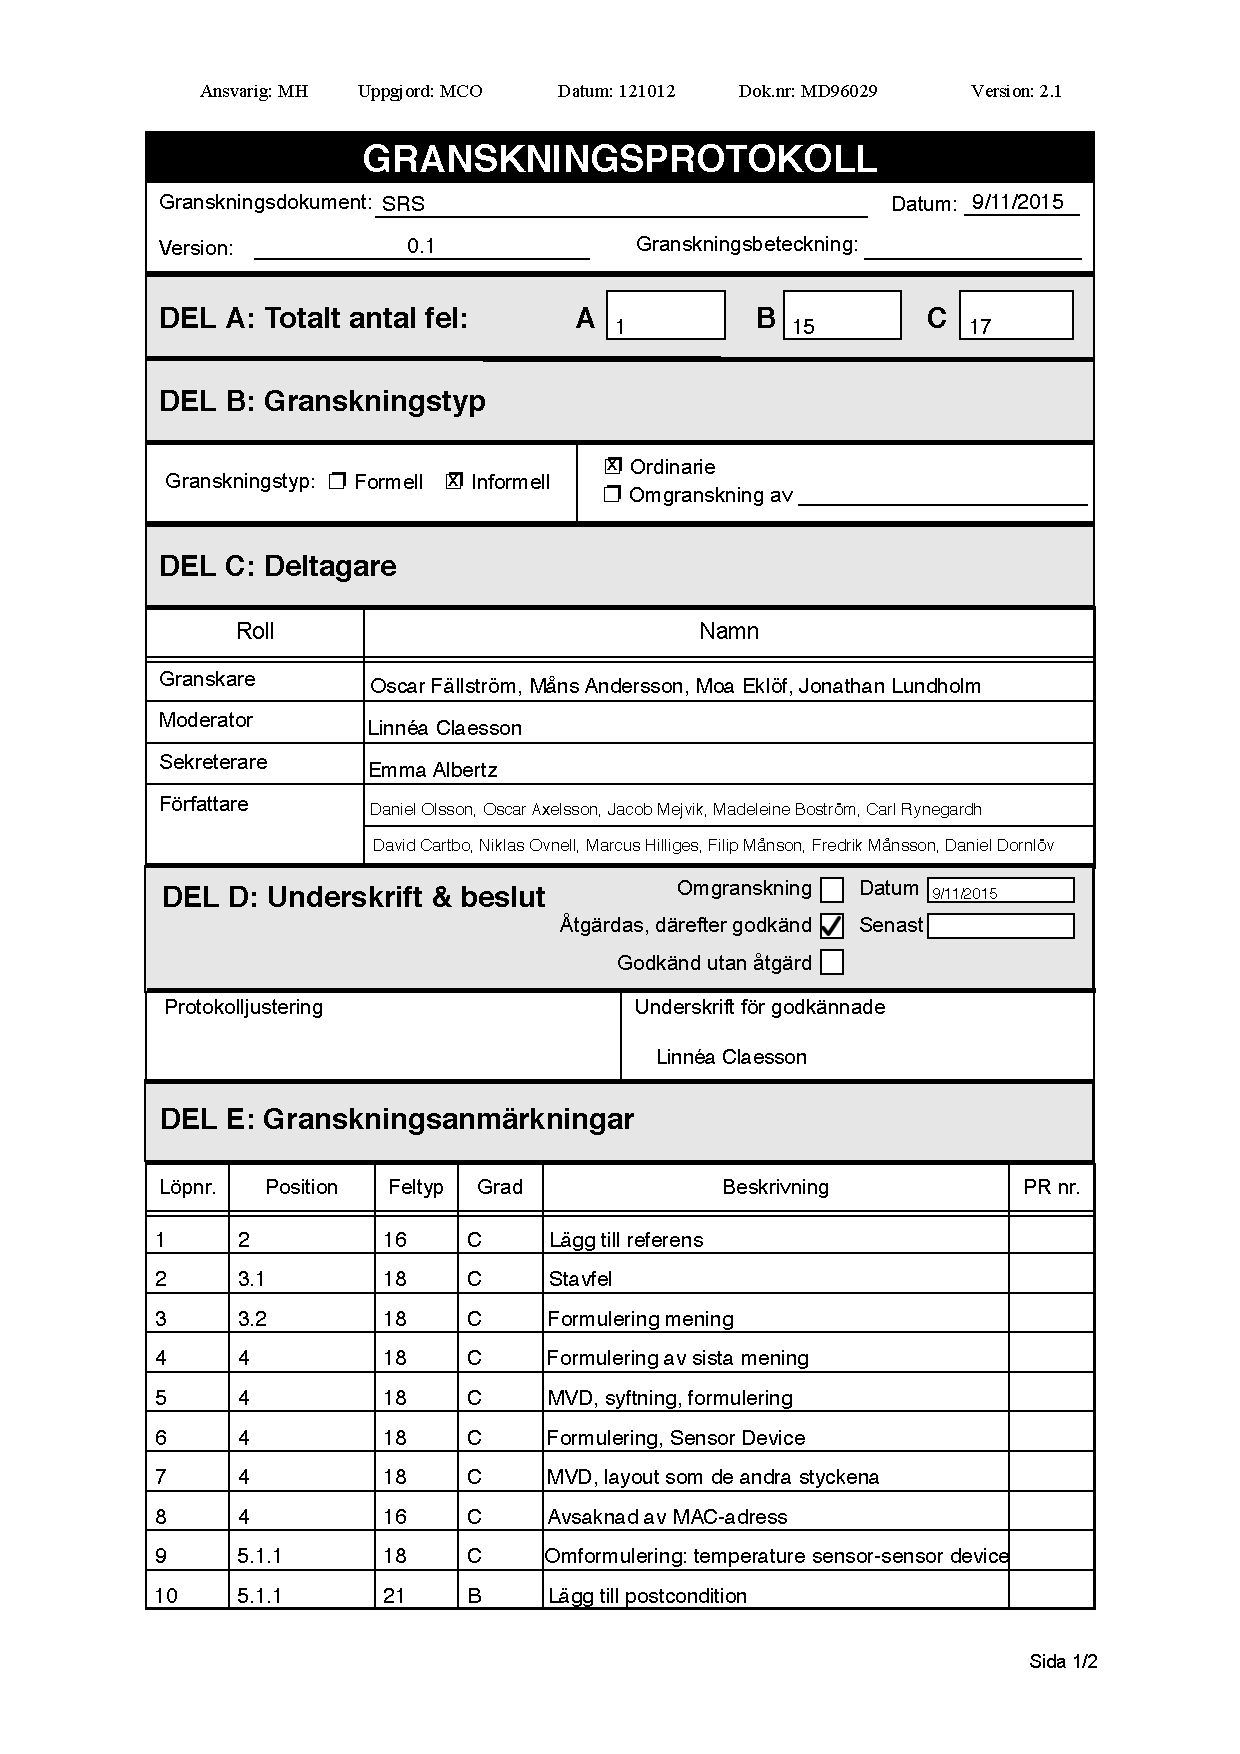
\includepdf[pages=-]{Reviews/Informal/Informal_Review_Protocol_SRS.pdf}
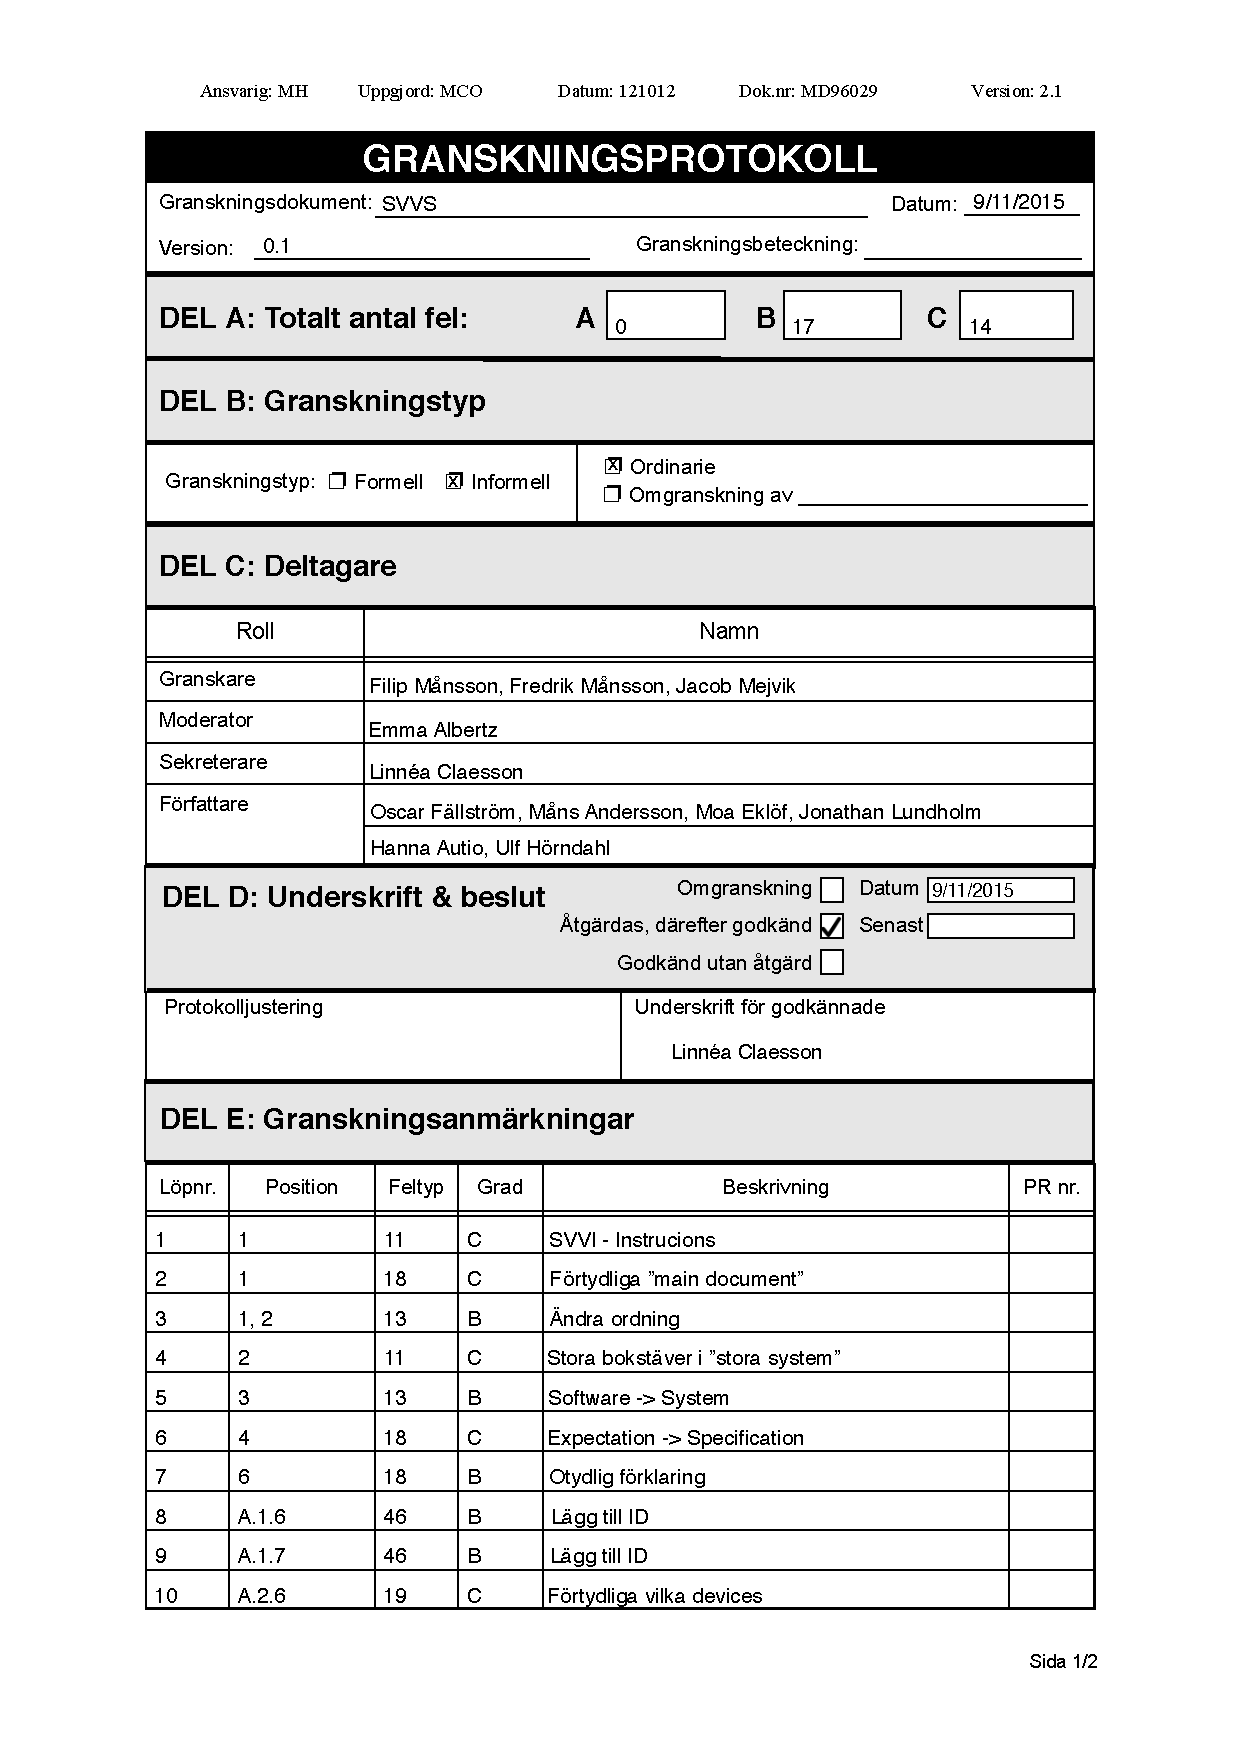
\includepdf[pages=-]{Reviews/Informal/Informal_Review_Protocol_SVVS.pdf}

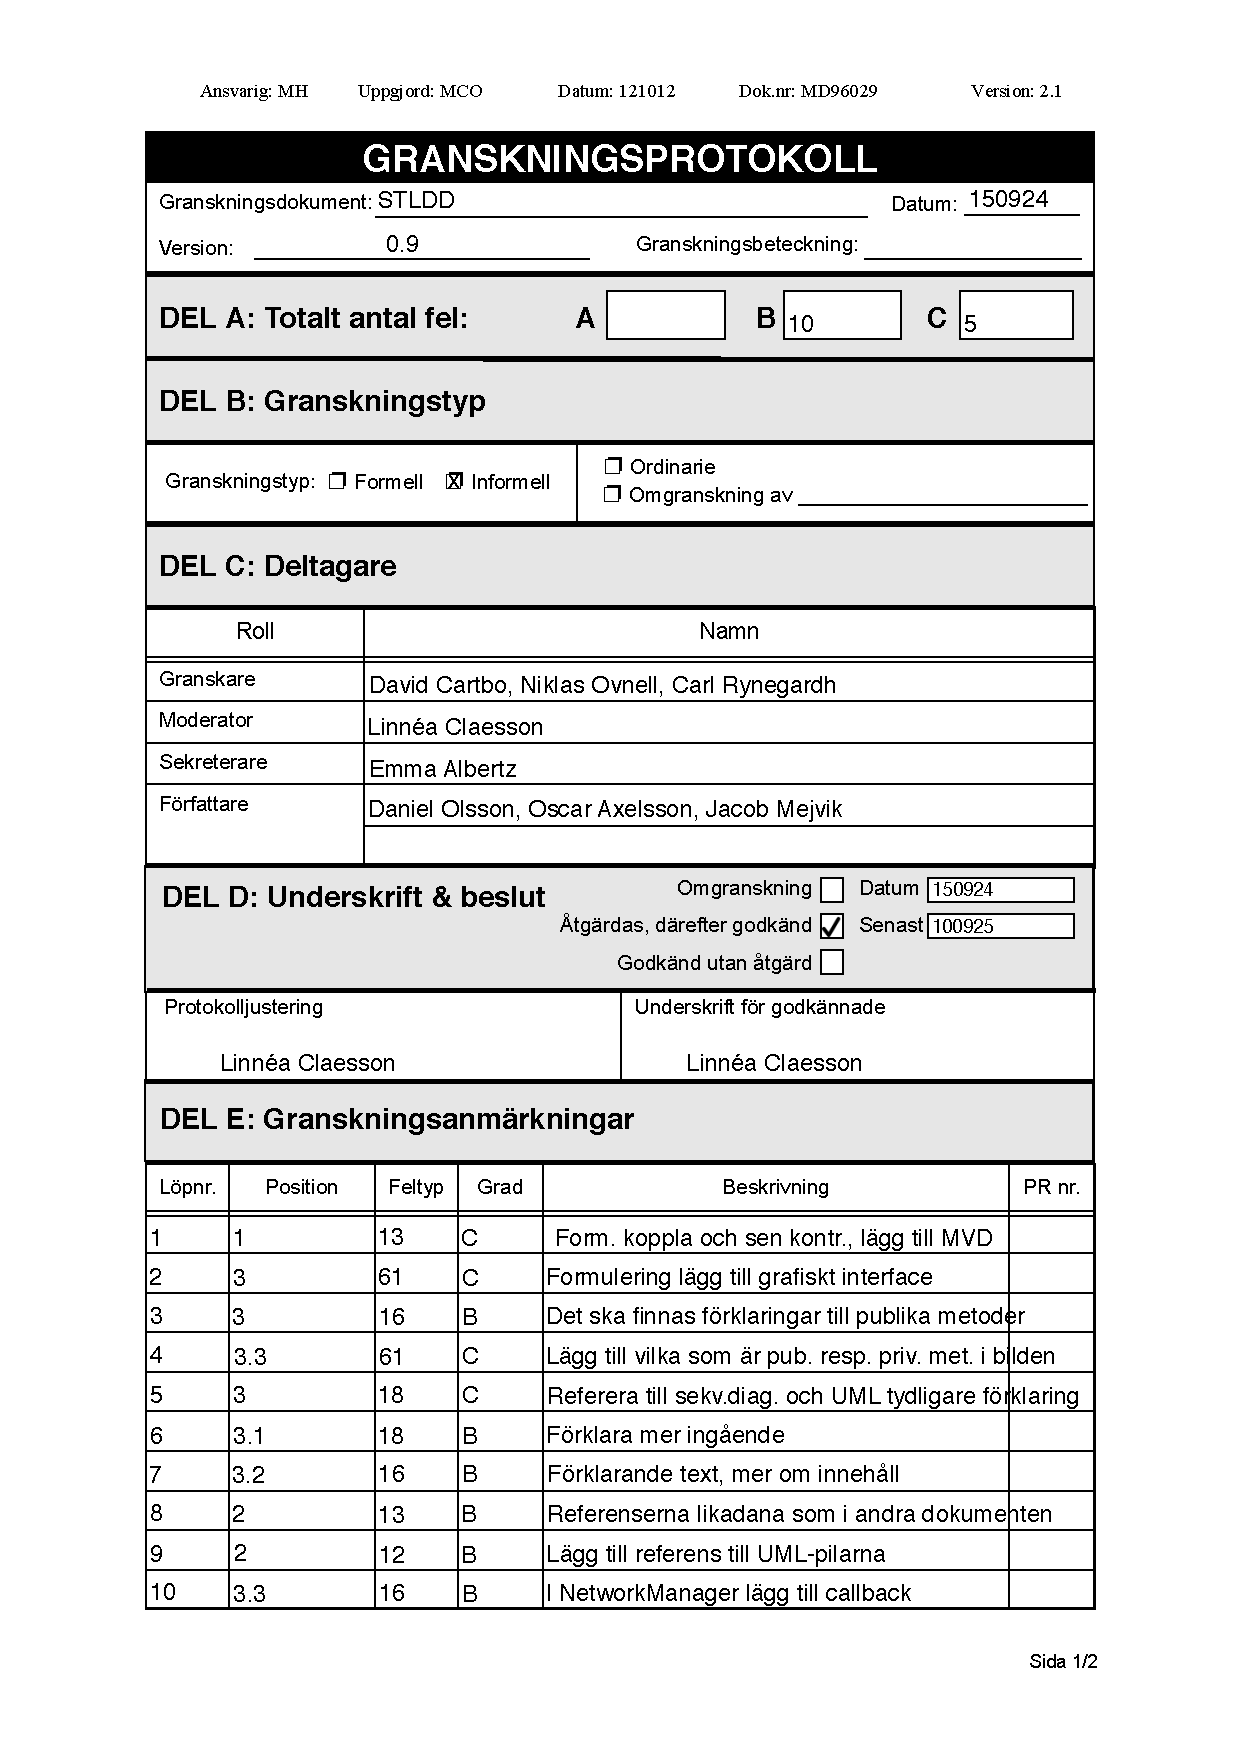
\includepdf[pages=-]{Reviews/Informal/Informal_Review_Protocol_STLDD.pdf}
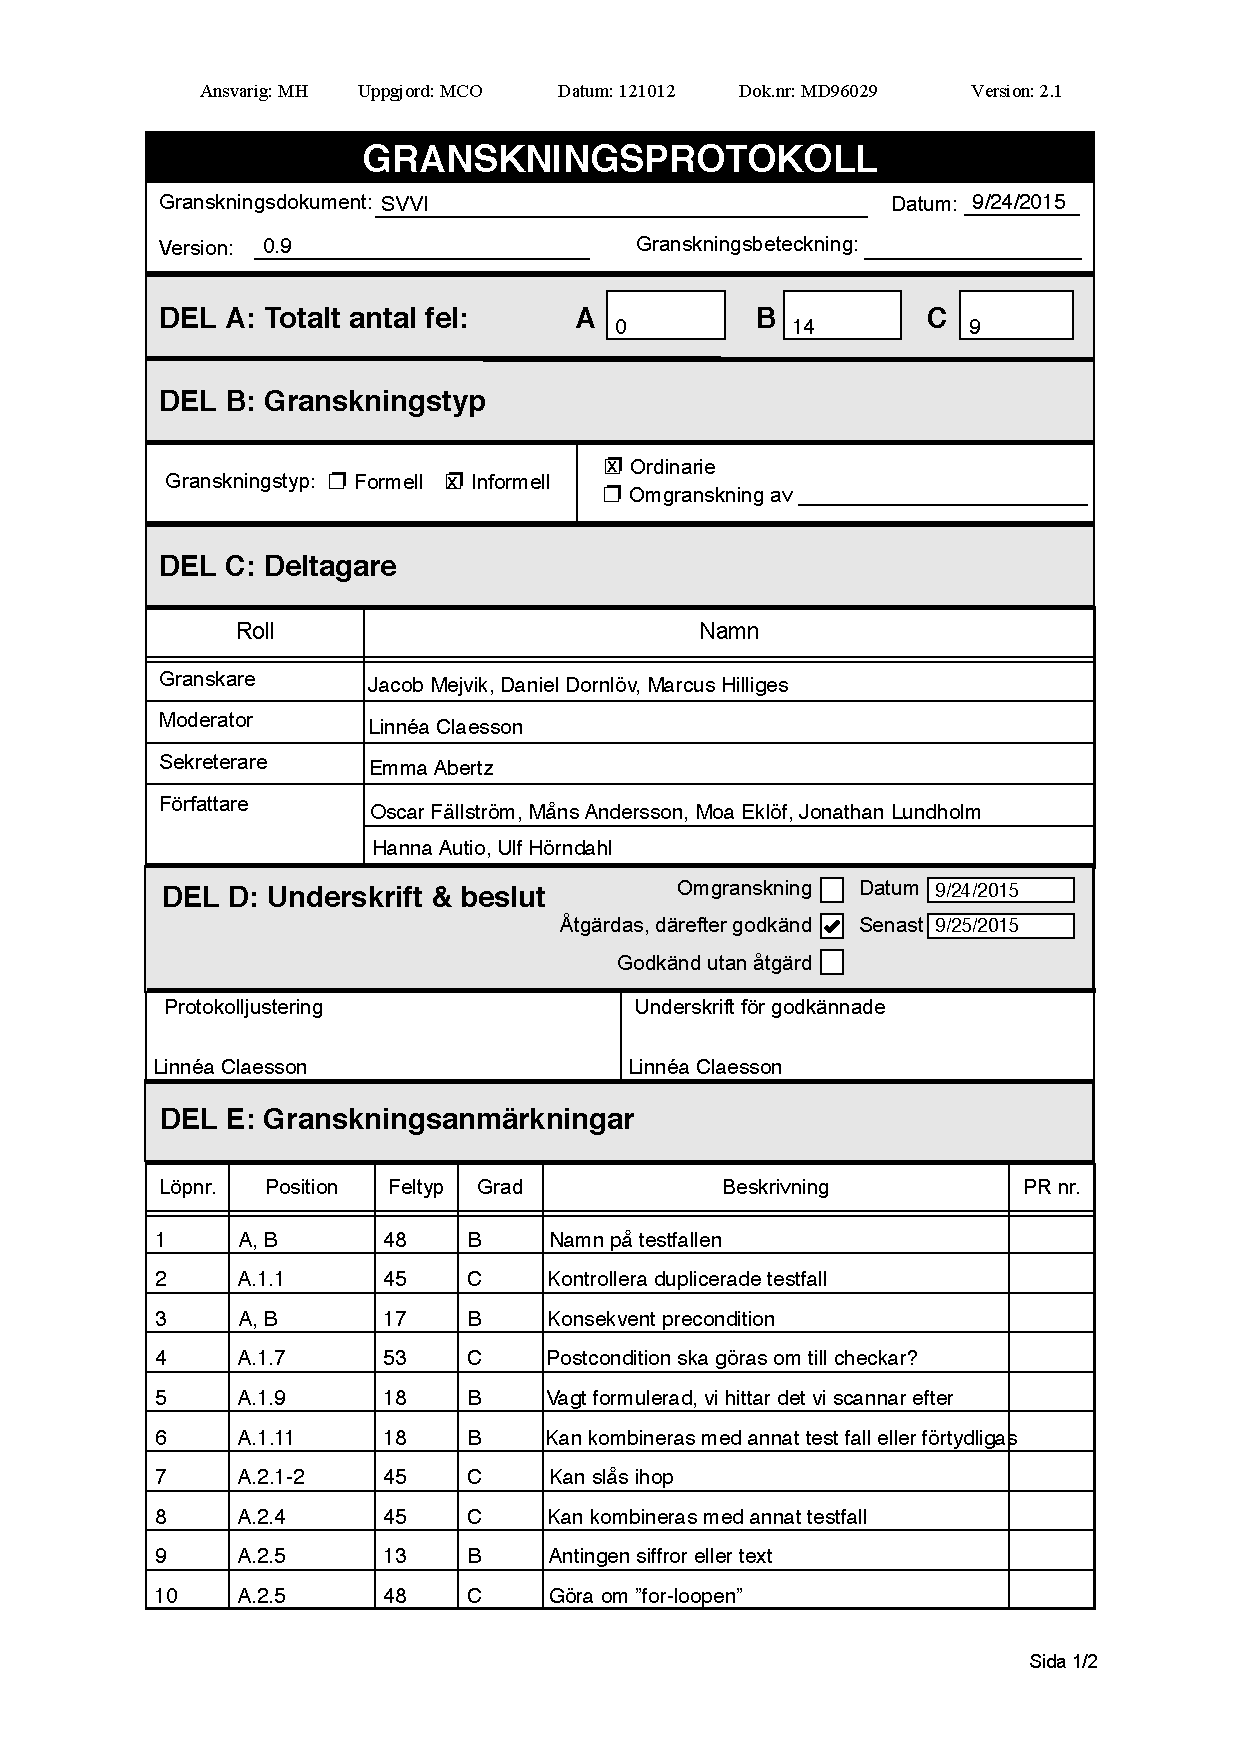
\includepdf[pages=-]{Reviews/Informal/Informal_Review_Protocol_SVVI.pdf}

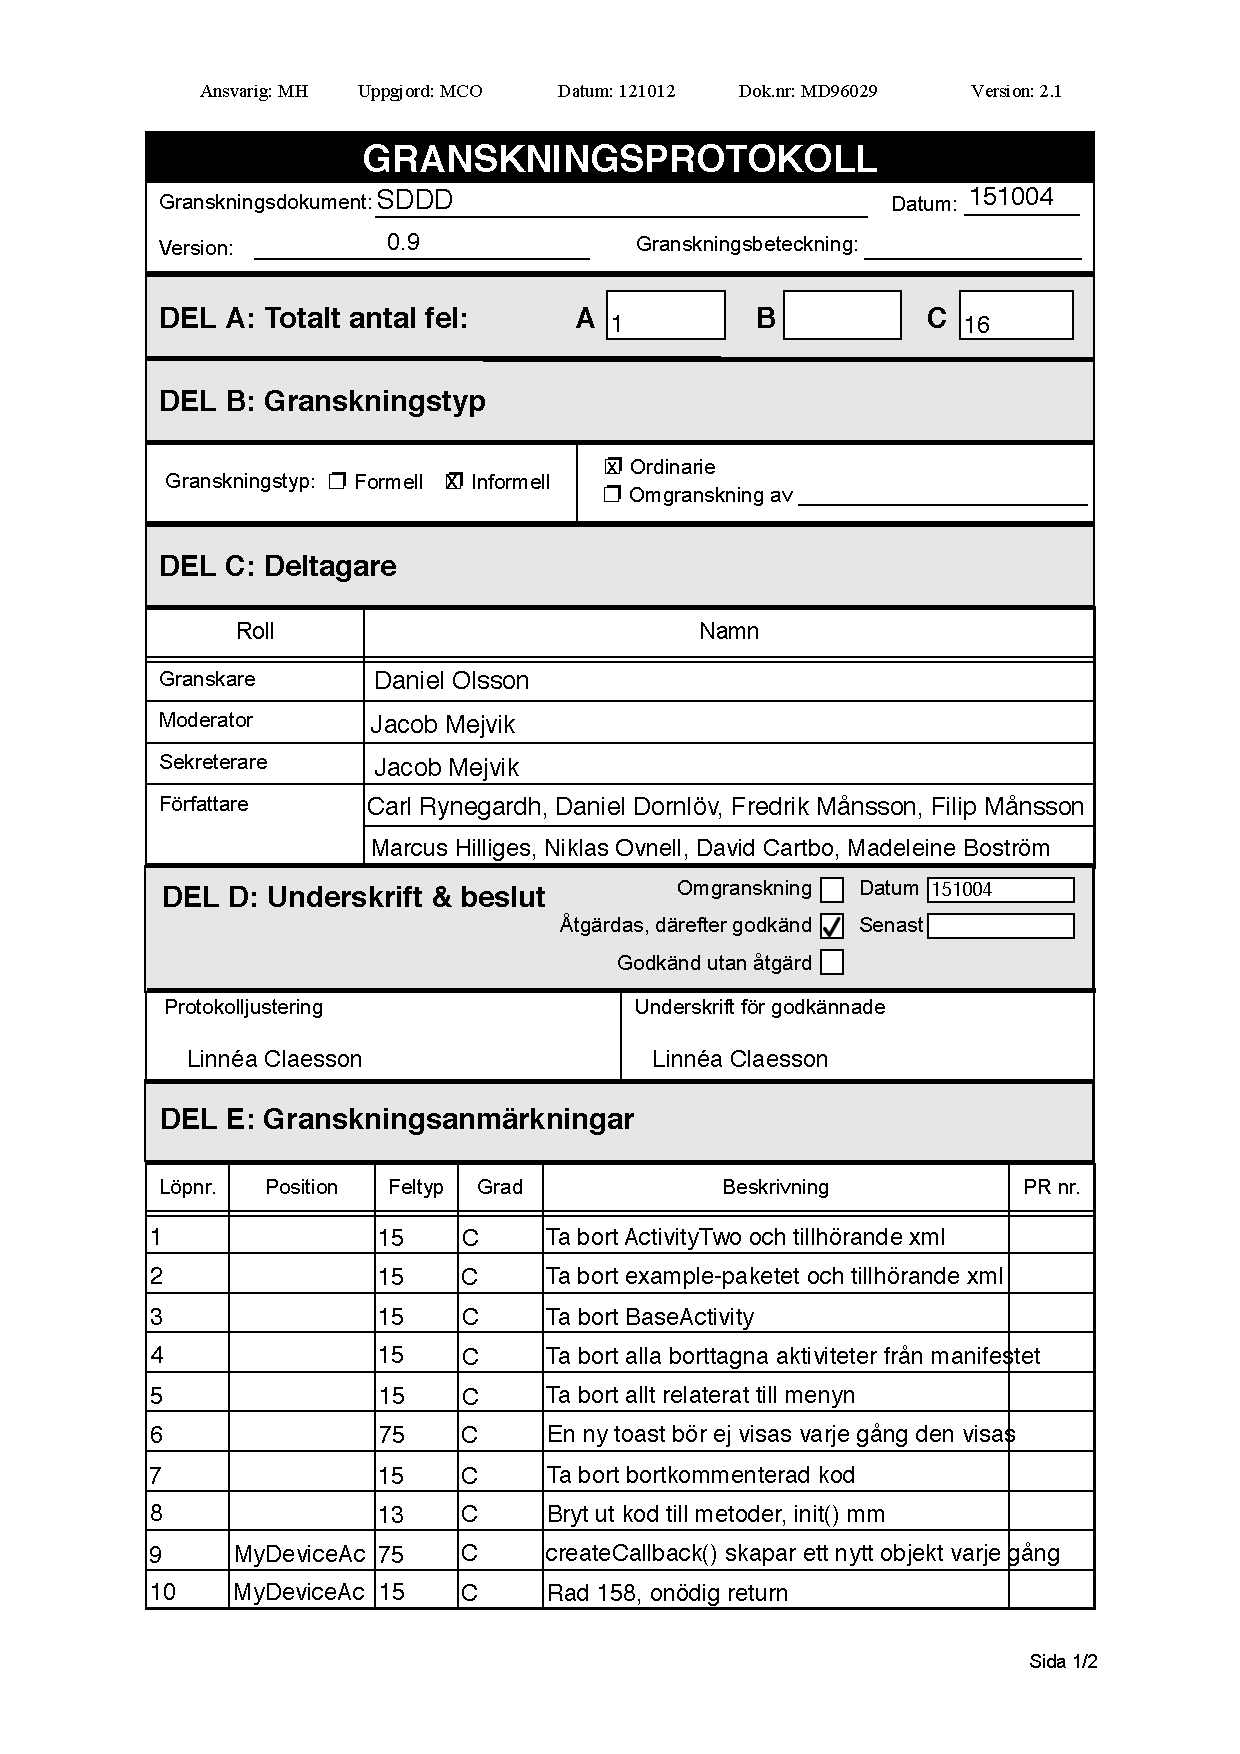
\includepdf[pages=-]{Reviews/Informal/Informal_Review_Protocol_SDDD.pdf}


\end{document}